\documentclass{article}
\usepackage[utf8]{inputenc}

\title{Visualizing a Highly Dimension Language Sound Space Using Cluster Analysis}
\author{Colby Ford, M.Sc.}
\date{2016}

\usepackage{natbib}
\usepackage{graphicx}

\begin{document}

\maketitle

\section{Methods}
To understand the relationship between different languages given their respective sound information, visualization is key for insight as to where the languages lie relative to one another. The visualization of the sound space of over 100 sounds (variables) is not straightforward as the maximum number of variables that can be plotted on a graph is limited to three. In order to reduce the dimensionality of the dataset down to a managable number, we have chosen to cluster the sounds into three groups. \cite{napoleon_pavalakodi_2011} \textit{See figure \ref{fig:vizworkflow}}.

\begin{figure}[h!]
\centering
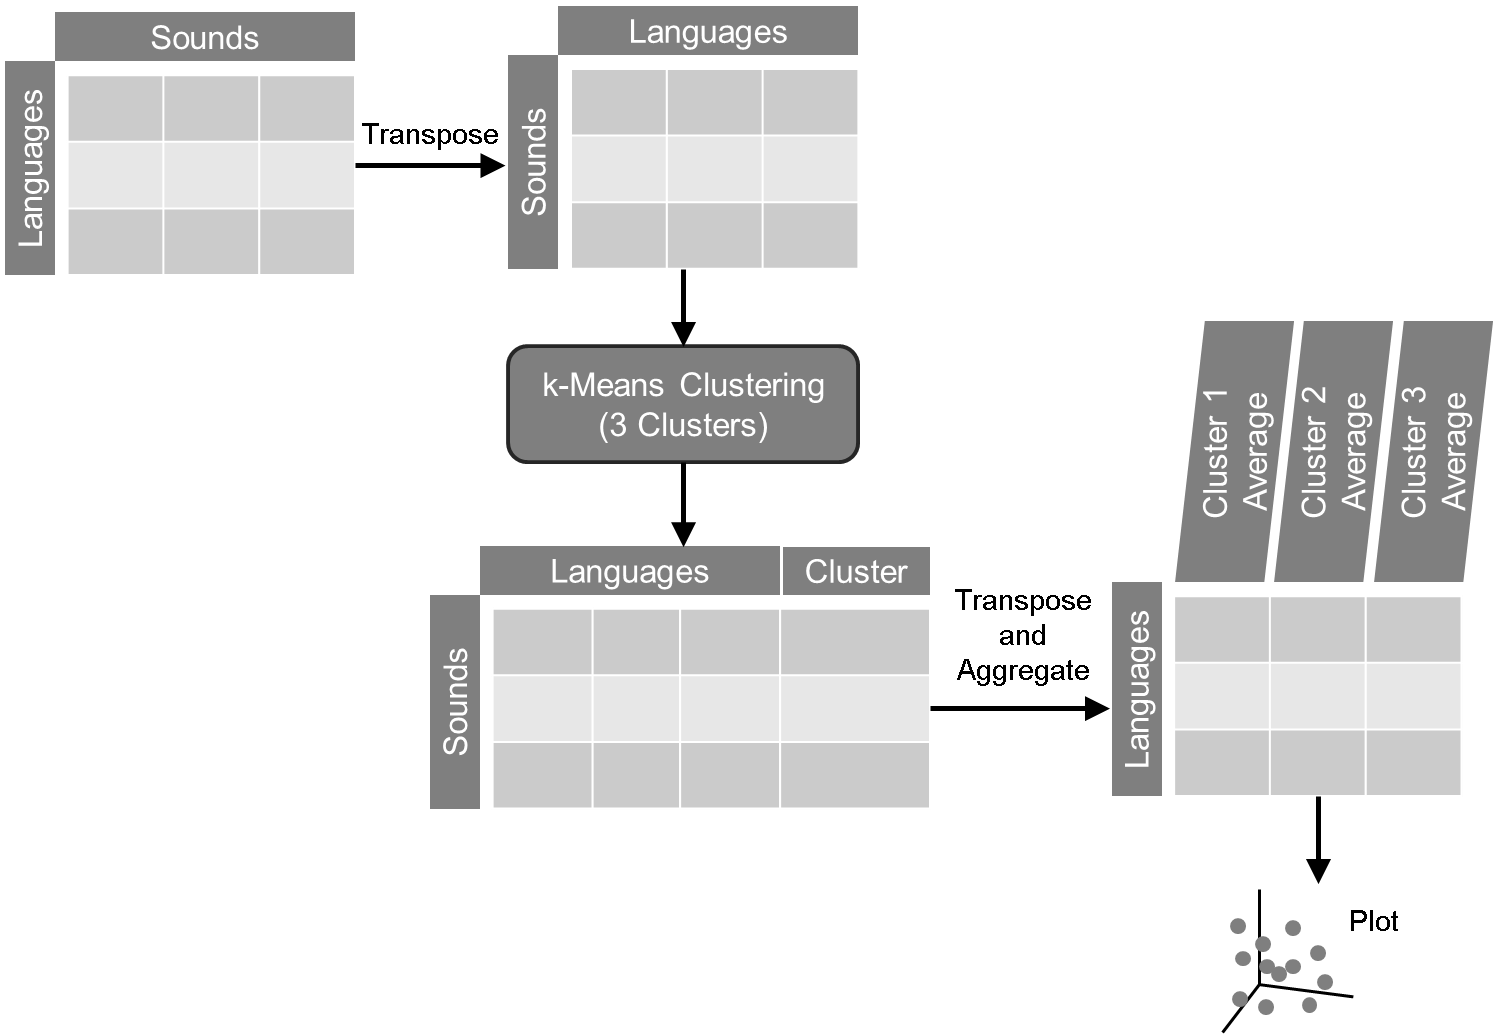
\includegraphics[width=\textwidth]{vizworkflow.png}
\caption{Analysis Workflow}
\label{fig:vizworkflow}
\end{figure}

%This analysis is done on two sets of languages: Uto-Aztecan and Bantu. For Uto-Aztecan, we have 141 sounds for 40 languages. For Bantu, we have 269 sounds for 105 languages.

k-Means clustering is the algorithm of choice. This method clusters variables into a set number of groups solely based on their mathematical distance from each other. In this case, the goal is to reduce the number of variables to plot from \>100 down to 3. By setting k = 3 in the algorithm, this will select 3 distinct clusters of sounds. \cite{mackay_2003}

\begin{figure}[h!]
\centering
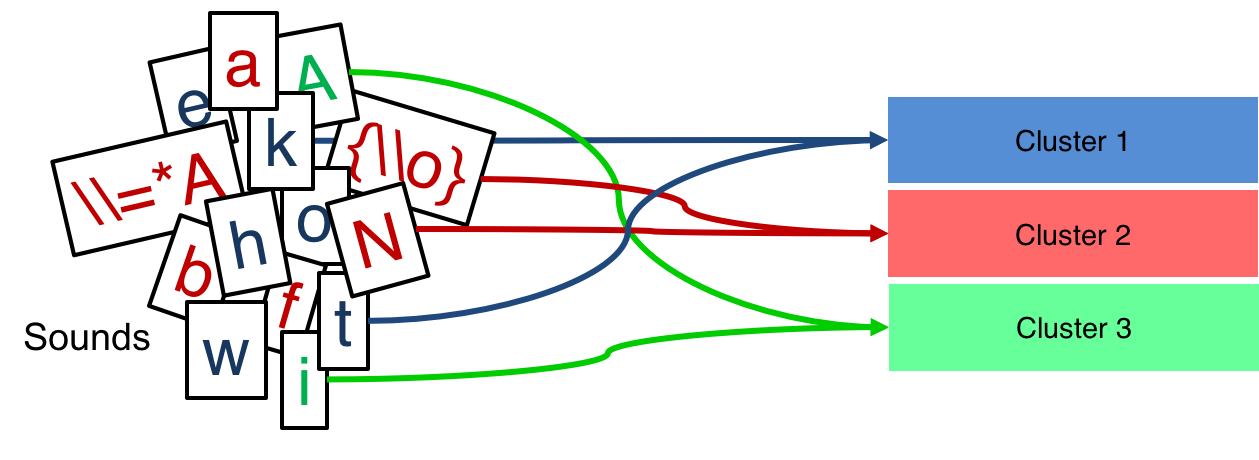
\includegraphics[width=\textwidth]{soundclusters.png}
\caption{Example of Sounds-Cluster Assignment}
\label{fig:soundclusters}
\end{figure}


The k-Means clustering algorithm generally treats rows as individual cases and columns as the variables to measure (the variables by which the distances are determined). The data is given as languages on rows and their sound values on columns. \textit{See table \ref{table:uadata_preT}}. This would mean that the analysis would group rows together based on the distances it found in the variables (columns). However, sounds are to be grouped, not languages. So, the data set is transposed to switch rows and columns. Once the data is transposed (\textit{See table \ref{table:uadata_postT}}), it is then passed to the k-Means algorithm, which is initialized using a random seed and set to run using 10,000 iterations to assure convergence. In other words, begin with a random set of variables and run through many iterations to make ensure the analysis is completed with all available data points.\cite{saseguide}

%Do we need to say what software was used? (SAS and Plot.ly)

\begin{table}
\centering
\begin{tabular}{|c| c c c c c|}
 \hline
 \multicolumn{6}{|c|}{\textbf{Uto-Aztecan Language Data}} \\
 \hline
 &\multicolumn{5}{|c|}{Sounds} \\
 \hline
 Language&A&B&...&T&W\\
 \hline
 Northern Paiute&0.143149284&0&...&0&8.18E-02\\
 Western Mono&0.105263158&0&...&0&6.24E-02\\
 Shoshone&0.125244618&0&...&0&0.105675147\\
 ...&...&...&...&...&...\\
 Pipil&0.108559499&0&..&0&0\\
 Kawaiisu&0.104065041&0&...&0&8.29E-02\\
 \hline
\end{tabular}
\caption{Original Data Format Example}
\label{table:uadata_preT}
\end{table}

\begin{table}
\centering
\begin{tabular}{|c| c c c c c c|}
 \hline
 \multicolumn{7}{|c|}{\textbf{Uto-Aztecan Language Data}} \\
 \hline
 &\multicolumn{6}{|c|}{Languages} \\
 \hline
 Sound&Northern Paiute&Western Mono&Shoshone&...&Pipil&Kawaiisu\\
 \hline
 A&0.143149284&0.105263158&0.125244618&...&0.108559499&0.104065041\\
 B&0&0&0&...&0&0\\
 ...&...&...&...&...&...&...\\
 T&0&0&0&...&0&0\\
 W&8.18E-02&6.24E-02&0.105675147&...&0&8.29E-02\\
 \hline
\end{tabular}
\caption{Transposed Data Format Example}
\label{table:uadata_postT}
\end{table}

The algorithm creates a new column with the cluster assignment for each sound. \textit{See table \ref{table:uadata_clust}}. This information is then pivoted to get the average values for each cluster of sounds per language. \textit{See table \ref{table:uadata_pivot}}. The last step is to use this information to plot the languages in 3-dimensional space with each of the clusters as an axis.\cite{plotly} \textit{See figure \ref{fig:uaplot1}}. The coordinates of the language points are the average values of all the sounds in each cluster.

\begin{table}
\centering
\begin{tabular}{|c| c |}
 \hline
 \multicolumn{2}{|c|}{\textbf{Uto-Aztecan Sound Cluster Assignments}} \\
 \hline
 Sound&Cluster\\
 \hline
 e&1\\
 h&1\\
 k&1\\
 ...&...\\
 g&2\\
 N&2\\
 ...&...\\
 A&3\\
 i&3\\
 \hline
\end{tabular}
\caption{Sound Cluster Assignment Example}
\label{table:uadata_clust}
\end{table}

\begin{table}
\centering
\begin{tabular}{|c| c c c |}
 \hline
 \multicolumn{4}{|c|}{\textbf{Uto-Aztecan Language Cluster Data}} \\
 \hline
 Language&Cluster 1&Cluster 2&Cluster 3\\
 \hline
 Northern Paiute&0.049590835&0.000676983&0.1255319\\
 Western Mono&0.046554648&0.001353356&0.093186373\\
 Shoshone&0.53861631&0.000444224&0.115694165\\
 ...&...&...&...\\
 Pipil&0.040556393&0.001542031&0.117647059\\
 Kawaiisu&0.045999227&0.001109443&0.115577889\\
 \hline
\end{tabular}
\caption{Pivoted Sound Cluster Data Example}
\label{table:uadata_pivot}
\end{table}

\begin{figure}[h!]
\centering
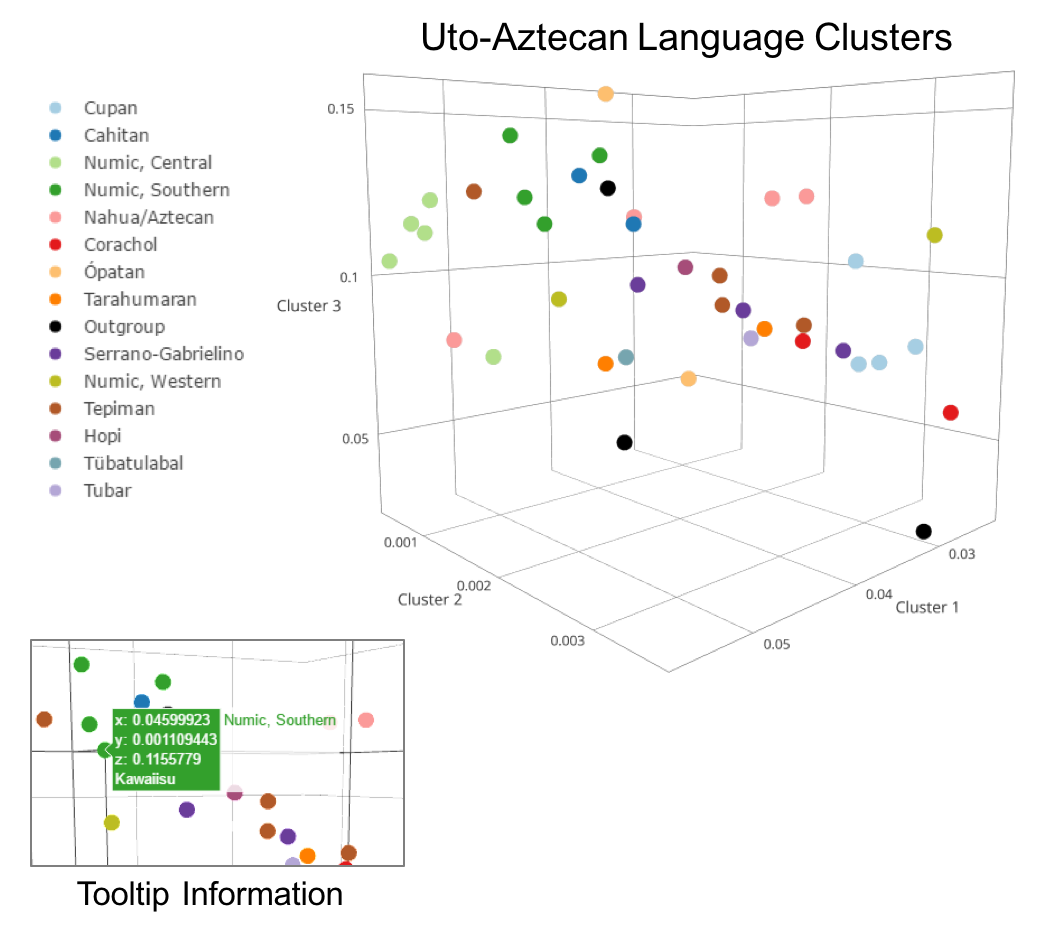
\includegraphics[width=\textwidth]{uaplot1.png}
\caption{Uto-Aztecan Language Plot}
\label{fig:uaplot1}
\end{figure}

\bibliographystyle{plain}
\bibliography{references}
\end{document}
